% Options for packages loaded elsewhere
\PassOptionsToPackage{unicode}{hyperref}
\PassOptionsToPackage{hyphens}{url}
%
\documentclass[
]{article}
\usepackage{amsmath,amssymb}
\usepackage{iftex}
\ifPDFTeX
  \usepackage[T1]{fontenc}
  \usepackage[utf8]{inputenc}
  \usepackage{textcomp} % provide euro and other symbols
\else % if luatex or xetex
  \usepackage{unicode-math} % this also loads fontspec
  \defaultfontfeatures{Scale=MatchLowercase}
  \defaultfontfeatures[\rmfamily]{Ligatures=TeX,Scale=1}
\fi
\usepackage{lmodern}
\ifPDFTeX\else
  % xetex/luatex font selection
\fi
% Use upquote if available, for straight quotes in verbatim environments
\IfFileExists{upquote.sty}{\usepackage{upquote}}{}
\IfFileExists{microtype.sty}{% use microtype if available
  \usepackage[]{microtype}
  \UseMicrotypeSet[protrusion]{basicmath} % disable protrusion for tt fonts
}{}
\makeatletter
\@ifundefined{KOMAClassName}{% if non-KOMA class
  \IfFileExists{parskip.sty}{%
    \usepackage{parskip}
  }{% else
    \setlength{\parindent}{0pt}
    \setlength{\parskip}{6pt plus 2pt minus 1pt}}
}{% if KOMA class
  \KOMAoptions{parskip=half}}
\makeatother
\usepackage{xcolor}
\usepackage[margin=1in]{geometry}
\usepackage{color}
\usepackage{fancyvrb}
\newcommand{\VerbBar}{|}
\newcommand{\VERB}{\Verb[commandchars=\\\{\}]}
\DefineVerbatimEnvironment{Highlighting}{Verbatim}{commandchars=\\\{\}}
% Add ',fontsize=\small' for more characters per line
\usepackage{framed}
\definecolor{shadecolor}{RGB}{248,248,248}
\newenvironment{Shaded}{\begin{snugshade}}{\end{snugshade}}
\newcommand{\AlertTok}[1]{\textcolor[rgb]{0.94,0.16,0.16}{#1}}
\newcommand{\AnnotationTok}[1]{\textcolor[rgb]{0.56,0.35,0.01}{\textbf{\textit{#1}}}}
\newcommand{\AttributeTok}[1]{\textcolor[rgb]{0.13,0.29,0.53}{#1}}
\newcommand{\BaseNTok}[1]{\textcolor[rgb]{0.00,0.00,0.81}{#1}}
\newcommand{\BuiltInTok}[1]{#1}
\newcommand{\CharTok}[1]{\textcolor[rgb]{0.31,0.60,0.02}{#1}}
\newcommand{\CommentTok}[1]{\textcolor[rgb]{0.56,0.35,0.01}{\textit{#1}}}
\newcommand{\CommentVarTok}[1]{\textcolor[rgb]{0.56,0.35,0.01}{\textbf{\textit{#1}}}}
\newcommand{\ConstantTok}[1]{\textcolor[rgb]{0.56,0.35,0.01}{#1}}
\newcommand{\ControlFlowTok}[1]{\textcolor[rgb]{0.13,0.29,0.53}{\textbf{#1}}}
\newcommand{\DataTypeTok}[1]{\textcolor[rgb]{0.13,0.29,0.53}{#1}}
\newcommand{\DecValTok}[1]{\textcolor[rgb]{0.00,0.00,0.81}{#1}}
\newcommand{\DocumentationTok}[1]{\textcolor[rgb]{0.56,0.35,0.01}{\textbf{\textit{#1}}}}
\newcommand{\ErrorTok}[1]{\textcolor[rgb]{0.64,0.00,0.00}{\textbf{#1}}}
\newcommand{\ExtensionTok}[1]{#1}
\newcommand{\FloatTok}[1]{\textcolor[rgb]{0.00,0.00,0.81}{#1}}
\newcommand{\FunctionTok}[1]{\textcolor[rgb]{0.13,0.29,0.53}{\textbf{#1}}}
\newcommand{\ImportTok}[1]{#1}
\newcommand{\InformationTok}[1]{\textcolor[rgb]{0.56,0.35,0.01}{\textbf{\textit{#1}}}}
\newcommand{\KeywordTok}[1]{\textcolor[rgb]{0.13,0.29,0.53}{\textbf{#1}}}
\newcommand{\NormalTok}[1]{#1}
\newcommand{\OperatorTok}[1]{\textcolor[rgb]{0.81,0.36,0.00}{\textbf{#1}}}
\newcommand{\OtherTok}[1]{\textcolor[rgb]{0.56,0.35,0.01}{#1}}
\newcommand{\PreprocessorTok}[1]{\textcolor[rgb]{0.56,0.35,0.01}{\textit{#1}}}
\newcommand{\RegionMarkerTok}[1]{#1}
\newcommand{\SpecialCharTok}[1]{\textcolor[rgb]{0.81,0.36,0.00}{\textbf{#1}}}
\newcommand{\SpecialStringTok}[1]{\textcolor[rgb]{0.31,0.60,0.02}{#1}}
\newcommand{\StringTok}[1]{\textcolor[rgb]{0.31,0.60,0.02}{#1}}
\newcommand{\VariableTok}[1]{\textcolor[rgb]{0.00,0.00,0.00}{#1}}
\newcommand{\VerbatimStringTok}[1]{\textcolor[rgb]{0.31,0.60,0.02}{#1}}
\newcommand{\WarningTok}[1]{\textcolor[rgb]{0.56,0.35,0.01}{\textbf{\textit{#1}}}}
\usepackage{graphicx}
\makeatletter
\def\maxwidth{\ifdim\Gin@nat@width>\linewidth\linewidth\else\Gin@nat@width\fi}
\def\maxheight{\ifdim\Gin@nat@height>\textheight\textheight\else\Gin@nat@height\fi}
\makeatother
% Scale images if necessary, so that they will not overflow the page
% margins by default, and it is still possible to overwrite the defaults
% using explicit options in \includegraphics[width, height, ...]{}
\setkeys{Gin}{width=\maxwidth,height=\maxheight,keepaspectratio}
% Set default figure placement to htbp
\makeatletter
\def\fps@figure{htbp}
\makeatother
\setlength{\emergencystretch}{3em} % prevent overfull lines
\providecommand{\tightlist}{%
  \setlength{\itemsep}{0pt}\setlength{\parskip}{0pt}}
\setcounter{secnumdepth}{-\maxdimen} % remove section numbering
\ifLuaTeX
  \usepackage{selnolig}  % disable illegal ligatures
\fi
\IfFileExists{bookmark.sty}{\usepackage{bookmark}}{\usepackage{hyperref}}
\IfFileExists{xurl.sty}{\usepackage{xurl}}{} % add URL line breaks if available
\urlstyle{same}
\hypersetup{
  hidelinks,
  pdfcreator={LaTeX via pandoc}}

\author{}
\date{\vspace{-2.5em}}

\begin{document}

\begin{Shaded}
\begin{Highlighting}[]
\CommentTok{\# Run data wrangling files first \#\#\#\#}
\CommentTok{\# Run limited service script}
\FunctionTok{source}\NormalTok{(}\AttributeTok{file =} \StringTok{"limited\_serv\_wrangling.R"}\NormalTok{, }\AttributeTok{local =}\NormalTok{ wrangled }\OtherTok{\textless{}{-}} \FunctionTok{new.env}\NormalTok{())}
\end{Highlighting}
\end{Shaded}

\begin{verbatim}
## Joining with `by = join_by(year, state)`
## Joining with `by = join_by(year, date, state, min_wage)`
\end{verbatim}

\begin{Shaded}
\begin{Highlighting}[]
\CommentTok{\# Run all industries script}
\FunctionTok{source}\NormalTok{(}\AttributeTok{file =} \StringTok{"all\_industries\_data\_wrangling.R"}\NormalTok{, }\AttributeTok{local =}\NormalTok{ wrangled)}
\FunctionTok{library}\NormalTok{(dplyr)}
\end{Highlighting}
\end{Shaded}

\begin{Shaded}
\begin{Highlighting}[]
\CommentTok{\# getwd()}
\end{Highlighting}
\end{Shaded}

\hypertarget{joining-all-industries-and-limited-service}{%
\section{Joining all industries and limited
service}\label{joining-all-industries-and-limited-service}}

\begin{Shaded}
\begin{Highlighting}[]
\NormalTok{joined }\OtherTok{\textless{}{-}} \FunctionTok{new.env}\NormalTok{()}
\NormalTok{joined}\SpecialCharTok{$}\NormalTok{data }\OtherTok{\textless{}{-}} \FunctionTok{full\_join}\NormalTok{(}
  \AttributeTok{x =}\NormalTok{ wrangled}\SpecialCharTok{$}\NormalTok{min\_wage}\SpecialCharTok{$}\NormalTok{limited\_increase,}
  \AttributeTok{y =}\NormalTok{ wrangled}\SpecialCharTok{$}\NormalTok{all\_ind\_combined}\SpecialCharTok{$}\NormalTok{gather) }\SpecialCharTok{|\textgreater{}} 
  \FunctionTok{mutate}\NormalTok{(}
    \AttributeTok{proportion\_limited =}\NormalTok{ emplvl\_limited }\SpecialCharTok{/}\NormalTok{ emplvl\_all) }\SpecialCharTok{|\textgreater{}}
  \CommentTok{\# filter(proportion\_limited \textgreater{} 0 \& !is.infinite(proportion\_limited)) |\textgreater{} }
  \FunctionTok{na.omit}\NormalTok{() }\SpecialCharTok{|\textgreater{}}
  \FunctionTok{mutate}\NormalTok{(}
    \AttributeTok{area\_fips =} \FunctionTok{factor}\NormalTok{(area\_fips)}
\NormalTok{  ) }\SpecialCharTok{\%\textgreater{}\%}
  \FunctionTok{filter}\NormalTok{(emplvl\_limited }\SpecialCharTok{\textgreater{}} \DecValTok{0}\NormalTok{)}
\end{Highlighting}
\end{Shaded}

\begin{verbatim}
## Joining with `by = join_by(area_fips, year, qtr, area_title, own_title, month)`
\end{verbatim}

\hypertarget{diagnostics}{%
\section{Diagnostics}\label{diagnostics}}

\hypertarget{checking-if-there-are-any-zeros}{%
\section{Checking if there are any
zeros}\label{checking-if-there-are-any-zeros}}

\hypertarget{rangejoineddataproportion_limited}{%
\section{\texorpdfstring{range(joined\(data\)proportion\_limited)}{range(joineddataproportion\_limited)}}\label{rangejoineddataproportion_limited}}

\hypertarget{rangejoineddataemplvl_all}{%
\section{\texorpdfstring{range(joined\(data\)emplvl\_all)}{range(joineddataemplvl\_all)}}\label{rangejoineddataemplvl_all}}

\hypertarget{rangejoineddataemplvl_limited}{%
\section{\texorpdfstring{range(joined\(data\)emplvl\_limited)}{range(joineddataemplvl\_limited)}}\label{rangejoineddataemplvl_limited}}

\hypertarget{anyjoineddata-22-23-0-checking-how-many-times-each-county-appears-tablejoineddatayear-joineddataarea_title}{%
\section{\texorpdfstring{any(joined\(data[,-22:-23] == 0) # # Checking how many times each county appears # table(joined\)data\(year, joined\)data\$area\_title)}{any(joineddata{[},-22:-23{]} == 0) \# \# Checking how many times each county appears \# table(joineddatayear, joineddata\$area\_title)}}\label{anyjoineddata-22-23-0-checking-how-many-times-each-county-appears-tablejoineddatayear-joineddataarea_title}}

\hypertarget{write_csvx-joineddata-file-joined_data.csv-joined---new.env-joineddata---read_csvfile-joined_data.csv}{%
\section{\texorpdfstring{write\_csv(x =
joined\(data, file = "joined_data.csv") # joined <- new.env() # joined\)data
\textless- read\_csv(file =
``joined\_data.csv'')}{write\_csv(x = joineddata, file = "joined\_data.csv") \# joined \textless- new.env() \# joineddata \textless- read\_csv(file = ``joined\_data.csv'')}}\label{write_csvx-joineddata-file-joined_data.csv-joined---new.env-joineddata---read_csvfile-joined_data.csv}}

\hypertarget{creating-dummies}{%
\section{Creating dummies}\label{creating-dummies}}

\hypertarget{libraryfastdummies}{%
\section{library(fastDummies)}\label{libraryfastdummies}}

\begin{Shaded}
\begin{Highlighting}[]
\CommentTok{\#Setting up for 2011{-}2012}

\NormalTok{data\_2011\_2012 }\OtherTok{\textless{}{-}}\NormalTok{ joined}\SpecialCharTok{$}\NormalTok{data }\SpecialCharTok{|\textgreater{}} 
  \FunctionTok{filter}\NormalTok{(year\_decimal }\SpecialCharTok{\%in\%} \FunctionTok{seq}\NormalTok{(}\FloatTok{2011.5}\NormalTok{,}\FloatTok{2012.5}\NormalTok{, }\AttributeTok{by =} \DecValTok{1}\SpecialCharTok{/}\DecValTok{12}\NormalTok{)) }\SpecialCharTok{|\textgreater{}} 
  \FunctionTok{mutate}\NormalTok{(}\AttributeTok{year =} \FunctionTok{as.factor}\NormalTok{(year))}

\CommentTok{\#Regression for 2011{-}2012}

\NormalTok{model\_2011\_2012 }\OtherTok{\textless{}{-}} \FunctionTok{lm}\NormalTok{(}\AttributeTok{formula =}\NormalTok{ emplvl\_limited }\SpecialCharTok{\textasciitilde{}}\NormalTok{ state }\SpecialCharTok{*}\NormalTok{ year }\SpecialCharTok{+}\NormalTok{ emplvl\_all,}
   \AttributeTok{data =}\NormalTok{ data\_2011\_2012) }

\NormalTok{model\_2011\_2012}
\end{Highlighting}
\end{Shaded}

\begin{verbatim}
## 
## Call:
## lm(formula = emplvl_limited ~ state * year + emplvl_all, data = data_2011_2012)
## 
## Coefficients:
##      (Intercept)           stateMO          year2012        emplvl_all  
##        -236.6024          629.1915          127.2332            0.0307  
## stateMO:year2012  
##        -110.2617
\end{verbatim}

\begin{Shaded}
\begin{Highlighting}[]
\CommentTok{\#Setting up for 2012{-}2013}

\NormalTok{data\_2012\_2013 }\OtherTok{\textless{}{-}}\NormalTok{ joined}\SpecialCharTok{$}\NormalTok{data }\SpecialCharTok{|\textgreater{}} 
  \FunctionTok{filter}\NormalTok{(year\_decimal }\SpecialCharTok{\%in\%} \FunctionTok{seq}\NormalTok{(}\FloatTok{2012.5}\NormalTok{,}\FloatTok{2013.5}\NormalTok{, }\AttributeTok{by =} \DecValTok{1}\SpecialCharTok{/}\DecValTok{12}\NormalTok{)) }\SpecialCharTok{|\textgreater{}} 
  \FunctionTok{mutate}\NormalTok{(}\AttributeTok{year =} \FunctionTok{as.factor}\NormalTok{(year)) }\CommentTok{\#|\textgreater{} }
  \CommentTok{\# dummy\_columns(}
  \CommentTok{\#   select\_columns = c(\textquotesingle{}year\_decimal\textquotesingle{}, \textquotesingle{}state\textquotesingle{}), }
  \CommentTok{\#   remove\_first\_dummy = TRUE, }
  \CommentTok{\# ) |\textgreater{} }
  \CommentTok{\# rename(post = year\_2013, treat = state\_MO)}
\end{Highlighting}
\end{Shaded}

\hypertarget{write_csvx-data_2012_2013-file-data_2012_2013.csv}{%
\section{write\_csv(x = data\_2012\_2013, file =
``data\_2012\_2013.csv'')}\label{write_csvx-data_2012_2013-file-data_2012_2013.csv}}

\hypertarget{data_2012_2013---read_csvfile-data_2012_2013.csv}{%
\section{data\_2012\_2013 \textless- read\_csv(file =
``data\_2012\_2013.csv'')}\label{data_2012_2013---read_csvfile-data_2012_2013.csv}}

\hypertarget{checking-if-there-are-any-zeros-1}{%
\section{\# Checking if there are any
zeros}\label{checking-if-there-are-any-zeros-1}}

\hypertarget{rangedata_2012_2013proportion_limited-rangedata_2012_2013emplvl_all}{%
\section{\texorpdfstring{range(data\_2012\_2013\(proportion_limited) # range(data_2012_2013\)emplvl\_all)}{range(data\_2012\_2013proportion\_limited) \# range(data\_2012\_2013emplvl\_all)}}\label{rangedata_2012_2013proportion_limited-rangedata_2012_2013emplvl_all}}

\hypertarget{rangedata_2012_2013emplvl_limited-anydata_2012_2013-22-23-0-checking-how-many-times-each-county-appears-tabledata_2012_2013year-data_2012_2013area_title}{%
\section{\texorpdfstring{range(data\_2012\_2013\(emplvl_limited) # any(data_2012_2013[,-22:-23] == 0) # # Checking how many times each county appears # table(data_2012_2013\)year,
data\_2012\_2013\$area\_title)}{range(data\_2012\_2013emplvl\_limited) \# any(data\_2012\_2013{[},-22:-23{]} == 0) \# \# Checking how many times each county appears \# table(data\_2012\_2013year, data\_2012\_2013\$area\_title)}}\label{rangedata_2012_2013emplvl_limited-anydata_2012_2013-22-23-0-checking-how-many-times-each-county-appears-tabledata_2012_2013year-data_2012_2013area_title}}

\hypertarget{section-2}{%
\section{\#\#\#\#\#\#\#\#\#\#\#\#\#\#\#\#\#\#\#\#}\label{section-2}}

\hypertarget{d-i-d}{%
\section{\#\#\#\#\#\#\#D-i-D}\label{d-i-d}}

\hypertarget{section-3}{%
\section{\#\#\#\#\#\#\#\#\#\#\#\#\#\#\#\#\#\#\#\#}\label{section-3}}

\hypertarget{models---new.env}{%
\section{models \textless- new.env()}\label{models---new.env}}

\{r\} library(lfe)

felm\_proportion \textless- felm(proportion\_limited \textasciitilde{}
state * year, data = data\_2012\_2013)

summary(felm\_proportion)

felm\_all \textless- lm(emplvl\_limited \textasciitilde{}
emplvl\_all\emph{year}state, data = data\_2012\_2013)

summary(felm\_all)

felm\_cont\_treatment \textless- felm(emplvl\_limited \textasciitilde{}
min\_wage + emplvl\_all \textbar{} area\_title + date, data =
joined\$data)

\hypertarget{summaryfelm_cont_treatment}{%
\section{summary(felm\_cont\_treatment)}\label{summaryfelm_cont_treatment}}

lm\_cont\_treatment \textless- lm(emplvl\_limited \textasciitilde{}
min\_wage + emplvl\_all + area\_title + factor(date), data =
joined\$data)

\hypertarget{summarylm_cont_treatment}{%
\section{summary(lm\_cont\_treatment)}\label{summarylm_cont_treatment}}

\hypertarget{try-using-this-with-felm-xactdof-true}{%
\section{try using this with felm: xactDOF =
TRUE)}\label{try-using-this-with-felm-xactdof-true}}

\hypertarget{trying-without-fixed-effects}{%
\section{Trying without fixed
effects}\label{trying-without-fixed-effects}}

lm\_proportion \textless- lm(proportion\_limited \textasciitilde{} treat
* post, data = data\_2012\_2013)

summary(lm\_proportion)

\begin{Shaded}
\begin{Highlighting}[]
\CommentTok{\#Regression for 2012{-}2013}

\NormalTok{model\_2012\_2013 }\OtherTok{\textless{}{-}} \FunctionTok{lm}\NormalTok{(}\AttributeTok{formula =}\NormalTok{ emplvl\_limited }\SpecialCharTok{\textasciitilde{}}\NormalTok{ state }\SpecialCharTok{*}\NormalTok{ year }\SpecialCharTok{+}\NormalTok{ emplvl\_all,}
   \AttributeTok{data =}\NormalTok{ data\_2012\_2013) }

\NormalTok{model\_2012\_2013}
\end{Highlighting}
\end{Shaded}

\begin{verbatim}
## 
## Call:
## lm(formula = emplvl_limited ~ state * year + emplvl_all, data = data_2012_2013)
## 
## Coefficients:
##      (Intercept)           stateMO          year2013        emplvl_all  
##       -163.55541         549.00101          23.99582           0.03142  
## stateMO:year2013  
##          6.80687
\end{verbatim}

\begin{Shaded}
\begin{Highlighting}[]
\CommentTok{\# Setting up for 2013 {-} 2014}

\NormalTok{data\_2013\_2014 }\OtherTok{\textless{}{-}}\NormalTok{ joined}\SpecialCharTok{$}\NormalTok{data }\SpecialCharTok{|\textgreater{}} 
  \FunctionTok{filter}\NormalTok{(year\_decimal }\SpecialCharTok{\%in\%} \FunctionTok{seq}\NormalTok{(}\FloatTok{2013.5}\NormalTok{,}\FloatTok{2014.5}\NormalTok{, }\AttributeTok{by =} \DecValTok{1}\SpecialCharTok{/}\DecValTok{12}\NormalTok{)) }\SpecialCharTok{|\textgreater{}} 
  \FunctionTok{mutate}\NormalTok{(}\AttributeTok{year =} \FunctionTok{as.factor}\NormalTok{(year))}

\CommentTok{\#Regression for 2013 {-} 2014}

\NormalTok{model\_2013\_2014 }\OtherTok{\textless{}{-}} \FunctionTok{lm}\NormalTok{(}\AttributeTok{formula =}\NormalTok{ emplvl\_limited }\SpecialCharTok{\textasciitilde{}}\NormalTok{ state }\SpecialCharTok{*}\NormalTok{ year }\SpecialCharTok{+}\NormalTok{ emplvl\_all,}
   \AttributeTok{data =}\NormalTok{ data\_2013\_2014) }

\NormalTok{model\_2013\_2014}
\end{Highlighting}
\end{Shaded}

\begin{verbatim}
## 
## Call:
## lm(formula = emplvl_limited ~ state * year + emplvl_all, data = data_2013_2014)
## 
## Coefficients:
##      (Intercept)           stateMO          year2014        emplvl_all  
##       -192.22233         596.56774         -32.31529           0.03182  
## stateMO:year2014  
##         94.41454
\end{verbatim}

\begin{Shaded}
\begin{Highlighting}[]
\CommentTok{\# Setting up for 2014 {-} 2015}

\NormalTok{data\_2014\_2015 }\OtherTok{\textless{}{-}}\NormalTok{ joined}\SpecialCharTok{$}\NormalTok{data }\SpecialCharTok{|\textgreater{}} 
  \FunctionTok{filter}\NormalTok{(year\_decimal }\SpecialCharTok{\%in\%} \FunctionTok{seq}\NormalTok{(}\FloatTok{2014.5}\NormalTok{,}\FloatTok{2015.5}\NormalTok{, }\AttributeTok{by =} \DecValTok{1}\SpecialCharTok{/}\DecValTok{12}\NormalTok{)) }\SpecialCharTok{|\textgreater{}} 
  \FunctionTok{mutate}\NormalTok{(}\AttributeTok{year =} \FunctionTok{as.factor}\NormalTok{(year))}

\CommentTok{\#Regression for 2014 {-} 2015}

\NormalTok{model\_2014\_2015 }\OtherTok{\textless{}{-}} \FunctionTok{lm}\NormalTok{(}\AttributeTok{formula =}\NormalTok{ emplvl\_limited }\SpecialCharTok{\textasciitilde{}}\NormalTok{ state }\SpecialCharTok{*}\NormalTok{ year }\SpecialCharTok{+}\NormalTok{ emplvl\_all,}
   \AttributeTok{data =}\NormalTok{ data\_2014\_2015) }

\NormalTok{model\_2014\_2015}
\end{Highlighting}
\end{Shaded}

\begin{verbatim}
## 
## Call:
## lm(formula = emplvl_limited ~ state * year + emplvl_all, data = data_2014_2015)
## 
## Coefficients:
##      (Intercept)           stateMO          year2015        emplvl_all  
##       -253.57132         695.80845          11.11175           0.03191  
## stateMO:year2015  
##         75.99156
\end{verbatim}

\begin{Shaded}
\begin{Highlighting}[]
\CommentTok{\# Setting up for 2015 {-} 2016}

\NormalTok{data\_2015\_2016 }\OtherTok{\textless{}{-}}\NormalTok{ joined}\SpecialCharTok{$}\NormalTok{data }\SpecialCharTok{|\textgreater{}} 
  \FunctionTok{filter}\NormalTok{(year\_decimal }\SpecialCharTok{\%in\%} \FunctionTok{seq}\NormalTok{(}\FloatTok{2015.5}\NormalTok{,}\FloatTok{2016.5}\NormalTok{, }\AttributeTok{by =} \DecValTok{1}\SpecialCharTok{/}\DecValTok{12}\NormalTok{)) }\SpecialCharTok{|\textgreater{}} 
  \FunctionTok{mutate}\NormalTok{(}\AttributeTok{year =} \FunctionTok{as.factor}\NormalTok{(year))}

\CommentTok{\#Regression for 2015 {-} 2016}

\NormalTok{model\_2015\_2016 }\OtherTok{\textless{}{-}} \FunctionTok{lm}\NormalTok{(}\AttributeTok{formula =}\NormalTok{ emplvl\_limited }\SpecialCharTok{\textasciitilde{}}\NormalTok{ state }\SpecialCharTok{*}\NormalTok{ year }\SpecialCharTok{+}\NormalTok{ emplvl\_all,}
   \AttributeTok{data =}\NormalTok{ data\_2015\_2016) }

\NormalTok{model\_2015\_2016}
\end{Highlighting}
\end{Shaded}

\begin{verbatim}
## 
## Call:
## lm(formula = emplvl_limited ~ state * year + emplvl_all, data = data_2015_2016)
## 
## Coefficients:
##      (Intercept)           stateMO          year2016        emplvl_all  
##       -312.90916         824.37573         133.01575           0.03246  
## stateMO:year2016  
##       -102.88055
\end{verbatim}

\begin{Shaded}
\begin{Highlighting}[]
\CommentTok{\# Setting up for 2016 {-} 2017}

\NormalTok{data\_2016\_2017 }\OtherTok{\textless{}{-}}\NormalTok{ joined}\SpecialCharTok{$}\NormalTok{data }\SpecialCharTok{|\textgreater{}} 
  \FunctionTok{filter}\NormalTok{(year\_decimal }\SpecialCharTok{\%in\%} \FunctionTok{seq}\NormalTok{(}\FloatTok{2016.5}\NormalTok{,}\FloatTok{2017.5}\NormalTok{, }\AttributeTok{by =} \DecValTok{1}\SpecialCharTok{/}\DecValTok{12}\NormalTok{)) }\SpecialCharTok{|\textgreater{}} 
  \FunctionTok{mutate}\NormalTok{(}\AttributeTok{year =} \FunctionTok{as.factor}\NormalTok{(year))}

\CommentTok{\#Regression for 2016 {-} 2017}

\NormalTok{model\_2016\_2017 }\OtherTok{\textless{}{-}} \FunctionTok{lm}\NormalTok{(}\AttributeTok{formula =}\NormalTok{ emplvl\_limited }\SpecialCharTok{\textasciitilde{}}\NormalTok{ state }\SpecialCharTok{*}\NormalTok{ year }\SpecialCharTok{+}\NormalTok{ emplvl\_all,}
   \AttributeTok{data =}\NormalTok{ data\_2016\_2017) }

\NormalTok{model\_2016\_2017}
\end{Highlighting}
\end{Shaded}

\begin{verbatim}
## 
## Call:
## lm(formula = emplvl_limited ~ state * year + emplvl_all, data = data_2016_2017)
## 
## Coefficients:
##      (Intercept)           stateMO          year2017        emplvl_all  
##       -237.26757         716.77097          66.42958           0.03276  
## stateMO:year2017  
##          7.61472
\end{verbatim}

\begin{Shaded}
\begin{Highlighting}[]
\CommentTok{\# Setting up for 2017 {-} 2018}

\NormalTok{data\_2017\_2018 }\OtherTok{\textless{}{-}}\NormalTok{ joined}\SpecialCharTok{$}\NormalTok{data }\SpecialCharTok{|\textgreater{}} 
  \FunctionTok{filter}\NormalTok{(year\_decimal }\SpecialCharTok{\%in\%} \FunctionTok{seq}\NormalTok{(}\FloatTok{2017.5}\NormalTok{,}\FloatTok{2018.5}\NormalTok{, }\AttributeTok{by =} \DecValTok{1}\SpecialCharTok{/}\DecValTok{12}\NormalTok{)) }\SpecialCharTok{|\textgreater{}} 
  \FunctionTok{mutate}\NormalTok{(}\AttributeTok{year =} \FunctionTok{as.factor}\NormalTok{(year))}

\CommentTok{\#Regression for 2017 {-} 2018}

\NormalTok{model\_2017\_2018 }\OtherTok{\textless{}{-}} \FunctionTok{lm}\NormalTok{(}\AttributeTok{formula =}\NormalTok{ emplvl\_limited }\SpecialCharTok{\textasciitilde{}}\NormalTok{ state }\SpecialCharTok{*}\NormalTok{ year }\SpecialCharTok{+}\NormalTok{ emplvl\_all,}
   \AttributeTok{data =}\NormalTok{ data\_2017\_2018) }

\NormalTok{model\_2017\_2018}
\end{Highlighting}
\end{Shaded}

\begin{verbatim}
## 
## Call:
## lm(formula = emplvl_limited ~ state * year + emplvl_all, data = data_2017_2018)
## 
## Coefficients:
##      (Intercept)           stateMO          year2018        emplvl_all  
##       -168.57196         731.10541          23.47235           0.03204  
## stateMO:year2018  
##        -78.05045
\end{verbatim}

\begin{Shaded}
\begin{Highlighting}[]
\CommentTok{\# Setting up for 2018 {-} 2019}

\NormalTok{data\_2018\_2019 }\OtherTok{\textless{}{-}}\NormalTok{ joined}\SpecialCharTok{$}\NormalTok{data }\SpecialCharTok{|\textgreater{}} 
  \FunctionTok{filter}\NormalTok{(year\_decimal }\SpecialCharTok{\%in\%} \FunctionTok{seq}\NormalTok{(}\FloatTok{2018.5}\NormalTok{,}\FloatTok{2019.5}\NormalTok{, }\AttributeTok{by =} \DecValTok{1}\SpecialCharTok{/}\DecValTok{12}\NormalTok{)) }\SpecialCharTok{|\textgreater{}} 
  \FunctionTok{mutate}\NormalTok{(}\AttributeTok{year =} \FunctionTok{as.factor}\NormalTok{(year))}

\CommentTok{\#Regression for 2018 {-} 2019}

\NormalTok{model\_2018\_2019 }\OtherTok{\textless{}{-}} \FunctionTok{lm}\NormalTok{(}\AttributeTok{formula =}\NormalTok{ emplvl\_limited }\SpecialCharTok{\textasciitilde{}}\NormalTok{ state }\SpecialCharTok{*}\NormalTok{ year }\SpecialCharTok{+}\NormalTok{ emplvl\_all,}
   \AttributeTok{data =}\NormalTok{ data\_2018\_2019) }

\NormalTok{model\_2018\_2019}
\end{Highlighting}
\end{Shaded}

\begin{verbatim}
## 
## Call:
## lm(formula = emplvl_limited ~ state * year + emplvl_all, data = data_2018_2019)
## 
## Coefficients:
##      (Intercept)           stateMO          year2019        emplvl_all  
##        -146.2029          671.6272           44.1102            0.0313  
## stateMO:year2019  
##           3.5421
\end{verbatim}

\begin{Shaded}
\begin{Highlighting}[]
\CommentTok{\# Setting up for 2019 {-} 2020}

\NormalTok{data\_2019\_2020 }\OtherTok{\textless{}{-}}\NormalTok{ joined}\SpecialCharTok{$}\NormalTok{data }\SpecialCharTok{|\textgreater{}} 
  \FunctionTok{filter}\NormalTok{(year\_decimal }\SpecialCharTok{\%in\%} \FunctionTok{seq}\NormalTok{(}\FloatTok{2019.5}\NormalTok{,}\FloatTok{2020.5}\NormalTok{, }\AttributeTok{by =} \DecValTok{1}\SpecialCharTok{/}\DecValTok{12}\NormalTok{)) }\SpecialCharTok{|\textgreater{}} 
  \FunctionTok{mutate}\NormalTok{(}\AttributeTok{year =} \FunctionTok{as.factor}\NormalTok{(year))}

\CommentTok{\#Regression for 2019 {-} 2020}

\NormalTok{model\_2019\_2020 }\OtherTok{\textless{}{-}} \FunctionTok{lm}\NormalTok{(}\AttributeTok{formula =}\NormalTok{ emplvl\_limited }\SpecialCharTok{\textasciitilde{}}\NormalTok{ state }\SpecialCharTok{*}\NormalTok{ year }\SpecialCharTok{+}\NormalTok{ emplvl\_all,}
   \AttributeTok{data =}\NormalTok{ data\_2019\_2020) }

\NormalTok{model\_2019\_2020}
\end{Highlighting}
\end{Shaded}

\begin{verbatim}
## 
## Call:
## lm(formula = emplvl_limited ~ state * year + emplvl_all, data = data_2019_2020)
## 
## Coefficients:
##      (Intercept)           stateMO          year2020        emplvl_all  
##       -132.29968         698.26594          -6.16743           0.03176  
## stateMO:year2020  
##         28.62215
\end{verbatim}

\begin{Shaded}
\begin{Highlighting}[]
\CommentTok{\# Setting up for 2020 {-} 2021}

\NormalTok{data\_2020\_2021 }\OtherTok{\textless{}{-}}\NormalTok{ joined}\SpecialCharTok{$}\NormalTok{data }\SpecialCharTok{|\textgreater{}} 
  \FunctionTok{filter}\NormalTok{(year\_decimal }\SpecialCharTok{\%in\%} \FunctionTok{seq}\NormalTok{(}\FloatTok{2020.5}\NormalTok{,}\FloatTok{2021.5}\NormalTok{, }\AttributeTok{by =} \DecValTok{1}\SpecialCharTok{/}\DecValTok{12}\NormalTok{)) }\SpecialCharTok{|\textgreater{}} 
  \FunctionTok{mutate}\NormalTok{(}\AttributeTok{year =} \FunctionTok{as.factor}\NormalTok{(year))}

\CommentTok{\#Regression for 2020 {-} 2021}

\NormalTok{model\_2020\_2021 }\OtherTok{\textless{}{-}} \FunctionTok{lm}\NormalTok{(}\AttributeTok{formula =}\NormalTok{ emplvl\_limited }\SpecialCharTok{\textasciitilde{}}\NormalTok{ state }\SpecialCharTok{*}\NormalTok{ year }\SpecialCharTok{+}\NormalTok{ emplvl\_all,}
   \AttributeTok{data =}\NormalTok{ data\_2020\_2021)}

\NormalTok{model\_2020\_2021}
\end{Highlighting}
\end{Shaded}

\begin{verbatim}
## 
## Call:
## lm(formula = emplvl_limited ~ state * year + emplvl_all, data = data_2020_2021)
## 
## Coefficients:
##      (Intercept)           stateMO          year2021        emplvl_all  
##       -148.37479         807.29653         -29.56850           0.03162  
## stateMO:year2021  
##          4.47185
\end{verbatim}

\begin{Shaded}
\begin{Highlighting}[]
\CommentTok{\# Setting up for 2021 {-} 2022}

\NormalTok{data\_2021\_2022 }\OtherTok{\textless{}{-}}\NormalTok{ joined}\SpecialCharTok{$}\NormalTok{data }\SpecialCharTok{|\textgreater{}} 
  \FunctionTok{filter}\NormalTok{(year\_decimal }\SpecialCharTok{\%in\%} \FunctionTok{seq}\NormalTok{(}\FloatTok{2021.5}\NormalTok{,}\FloatTok{2022.5}\NormalTok{, }\AttributeTok{by =} \DecValTok{1}\SpecialCharTok{/}\DecValTok{12}\NormalTok{)) }\SpecialCharTok{|\textgreater{}} 
  \FunctionTok{mutate}\NormalTok{(}\AttributeTok{year =} \FunctionTok{as.factor}\NormalTok{(year))}

\CommentTok{\#Regression for 2021 {-} 2022}

\NormalTok{model\_2021\_2022 }\OtherTok{\textless{}{-}} \FunctionTok{lm}\NormalTok{(}\AttributeTok{formula =}\NormalTok{ emplvl\_limited }\SpecialCharTok{\textasciitilde{}}\NormalTok{ state }\SpecialCharTok{*}\NormalTok{ year }\SpecialCharTok{+}\NormalTok{ emplvl\_all,}
   \AttributeTok{data =}\NormalTok{ data\_2021\_2022) }

\NormalTok{model\_2021\_2022}
\end{Highlighting}
\end{Shaded}

\begin{verbatim}
## 
## Call:
## lm(formula = emplvl_limited ~ state * year + emplvl_all, data = data_2021_2022)
## 
## Coefficients:
##      (Intercept)           stateMO          year2022        emplvl_all  
##       -206.68180         850.16261          24.89593           0.03113  
## stateMO:year2022  
##         37.83004
\end{verbatim}

\begin{Shaded}
\begin{Highlighting}[]
\NormalTok{confint\_model\_2011\_2012 }\OtherTok{\textless{}{-}} \FunctionTok{confint}\NormalTok{(model\_2011\_2012)[}\StringTok{"stateMO:year2012"}\NormalTok{,]}
          
\NormalTok{confint\_model\_2012\_2013 }\OtherTok{\textless{}{-}} \FunctionTok{confint}\NormalTok{(model\_2012\_2013)[}\StringTok{"stateMO:year2013"}\NormalTok{,]}

\NormalTok{confint\_model\_2013\_2014 }\OtherTok{\textless{}{-}} \FunctionTok{confint}\NormalTok{(model\_2013\_2014)}
\NormalTok{confint\_model\_2014\_2015 }\OtherTok{\textless{}{-}} \FunctionTok{confint}\NormalTok{(model\_2014\_2015)}
\NormalTok{confint\_model\_2015\_2016 }\OtherTok{\textless{}{-}} \FunctionTok{confint}\NormalTok{(model\_2015\_2016)}
\NormalTok{confint\_model\_2016\_2017 }\OtherTok{\textless{}{-}} \FunctionTok{confint}\NormalTok{(model\_2016\_2017)}
\NormalTok{confint\_model\_2017\_2018 }\OtherTok{\textless{}{-}} \FunctionTok{confint}\NormalTok{(model\_2017\_2018)}
\NormalTok{confint\_model\_2018\_2019 }\OtherTok{\textless{}{-}} \FunctionTok{confint}\NormalTok{(model\_2018\_2019)}
\NormalTok{confint\_model\_2019\_2020 }\OtherTok{\textless{}{-}} \FunctionTok{confint}\NormalTok{(model\_2019\_2020)}
\NormalTok{confint\_model\_2020\_2021 }\OtherTok{\textless{}{-}} \FunctionTok{confint}\NormalTok{(model\_2020\_2021)}
\NormalTok{confint\_model\_2021\_2022 }\OtherTok{\textless{}{-}} \FunctionTok{confint}\NormalTok{(model\_2021\_2022)}
\end{Highlighting}
\end{Shaded}

\begin{Shaded}
\begin{Highlighting}[]
\NormalTok{confints }\OtherTok{\textless{}{-}} \FunctionTok{rbind}\NormalTok{(}
\StringTok{"m\_2012"} \OtherTok{=} \FunctionTok{confint}\NormalTok{(model\_2011\_2012)[}\StringTok{"stateMO:year2012"}\NormalTok{,], }\StringTok{"m\_2013"} \OtherTok{=} \FunctionTok{confint}\NormalTok{(model\_2012\_2013)[}\StringTok{"stateMO:year2013"}\NormalTok{,], }\StringTok{"m\_2014"} \OtherTok{=} \FunctionTok{confint}\NormalTok{(model\_2013\_2014)[}\StringTok{"stateMO:year2014"}\NormalTok{,], }\StringTok{"m\_2015"} \OtherTok{=} \FunctionTok{confint}\NormalTok{(model\_2014\_2015)[}\StringTok{"stateMO:year2015"}\NormalTok{,],}
\StringTok{"m\_2016"} \OtherTok{=} \FunctionTok{confint}\NormalTok{(model\_2015\_2016)[}\StringTok{"stateMO:year2016"}\NormalTok{,],}
\StringTok{"m\_2017"} \OtherTok{=} \FunctionTok{confint}\NormalTok{(model\_2016\_2017)[}\StringTok{"stateMO:year2017"}\NormalTok{,],}
\StringTok{"m\_2018"} \OtherTok{=} \FunctionTok{confint}\NormalTok{(model\_2017\_2018)[}\StringTok{"stateMO:year2018"}\NormalTok{,],}
\StringTok{"m\_2019"} \OtherTok{=} \FunctionTok{confint}\NormalTok{(model\_2018\_2019)[}\StringTok{"stateMO:year2019"}\NormalTok{,],}
\StringTok{"m\_2020"} \OtherTok{=} \FunctionTok{confint}\NormalTok{(model\_2019\_2020)[}\StringTok{"stateMO:year2020"}\NormalTok{,],}
\StringTok{"m\_2021"} \OtherTok{=} \FunctionTok{confint}\NormalTok{(model\_2020\_2021)[}\StringTok{"stateMO:year2021"}\NormalTok{,],}
\StringTok{"m\_2022"} \OtherTok{=} \FunctionTok{confint}\NormalTok{(model\_2021\_2022)[}\StringTok{"stateMO:year2022"}\NormalTok{,]}
\NormalTok{) }\SpecialCharTok{\%\textgreater{}\%} \FunctionTok{as.data.frame}\NormalTok{() }\SpecialCharTok{\%\textgreater{}\%}
  \FunctionTok{mutate}\NormalTok{(}\AttributeTok{year =} \DecValTok{2012}\SpecialCharTok{:}\DecValTok{2022}\NormalTok{)}
\end{Highlighting}
\end{Shaded}

\begin{Shaded}
\begin{Highlighting}[]
\CommentTok{\# Compile coefficients into dataframe for visualizations}

\FunctionTok{library}\NormalTok{(broom)}

\NormalTok{tidy\_model\_2011\_2012 }\OtherTok{\textless{}{-}} \FunctionTok{tidy}\NormalTok{(model\_2011\_2012) }\SpecialCharTok{\%\textgreater{}\%}
  \FunctionTok{filter}\NormalTok{(term }\SpecialCharTok{\%in\%} \StringTok{"stateMO:year2012"}\NormalTok{) }\SpecialCharTok{\%\textgreater{}\%}
           \FunctionTok{select}\NormalTok{(term,estimate)}

\NormalTok{tidy\_model\_2012\_2013 }\OtherTok{\textless{}{-}} \FunctionTok{tidy}\NormalTok{(model\_2012\_2013) }\SpecialCharTok{\%\textgreater{}\%}
  \FunctionTok{filter}\NormalTok{(term }\SpecialCharTok{\%in\%} \StringTok{"stateMO:year2013"}\NormalTok{) }\SpecialCharTok{\%\textgreater{}\%}
           \FunctionTok{select}\NormalTok{(term,estimate)}


\NormalTok{tidy\_model\_2013\_2014 }\OtherTok{\textless{}{-}} \FunctionTok{tidy}\NormalTok{(model\_2013\_2014) }\SpecialCharTok{\%\textgreater{}\%}
  \FunctionTok{filter}\NormalTok{(term }\SpecialCharTok{\%in\%} \StringTok{"stateMO:year2014"}\NormalTok{) }\SpecialCharTok{\%\textgreater{}\%}
           \FunctionTok{select}\NormalTok{(term,estimate)}

\NormalTok{tidy\_model\_2014\_2015 }\OtherTok{\textless{}{-}} \FunctionTok{tidy}\NormalTok{(model\_2014\_2015) }\SpecialCharTok{\%\textgreater{}\%}
  \FunctionTok{filter}\NormalTok{(term }\SpecialCharTok{\%in\%} \StringTok{"stateMO:year2015"}\NormalTok{) }\SpecialCharTok{\%\textgreater{}\%}
           \FunctionTok{select}\NormalTok{(term,estimate)}

\NormalTok{tidy\_model\_2015\_2016 }\OtherTok{\textless{}{-}} \FunctionTok{tidy}\NormalTok{(model\_2015\_2016) }\SpecialCharTok{\%\textgreater{}\%}
  \FunctionTok{filter}\NormalTok{(term }\SpecialCharTok{\%in\%} \StringTok{"stateMO:year2016"}\NormalTok{) }\SpecialCharTok{\%\textgreater{}\%}
           \FunctionTok{select}\NormalTok{(term,estimate)}

\NormalTok{tidy\_model\_2016\_2017 }\OtherTok{\textless{}{-}} \FunctionTok{tidy}\NormalTok{(model\_2016\_2017) }\SpecialCharTok{\%\textgreater{}\%}
  \FunctionTok{filter}\NormalTok{(term }\SpecialCharTok{\%in\%} \StringTok{"stateMO:year2017"}\NormalTok{) }\SpecialCharTok{\%\textgreater{}\%}
           \FunctionTok{select}\NormalTok{(term,estimate)}

\NormalTok{tidy\_model\_2017\_2018 }\OtherTok{\textless{}{-}} \FunctionTok{tidy}\NormalTok{(model\_2017\_2018) }\SpecialCharTok{\%\textgreater{}\%}
  \FunctionTok{filter}\NormalTok{(term }\SpecialCharTok{\%in\%} \StringTok{"stateMO:year2018"}\NormalTok{) }\SpecialCharTok{\%\textgreater{}\%}
           \FunctionTok{select}\NormalTok{(term,estimate)}

\NormalTok{tidy\_model\_2018\_2019 }\OtherTok{\textless{}{-}} \FunctionTok{tidy}\NormalTok{(model\_2018\_2019) }\SpecialCharTok{\%\textgreater{}\%}
  \FunctionTok{filter}\NormalTok{(term }\SpecialCharTok{\%in\%} \StringTok{"stateMO:year2019"}\NormalTok{) }\SpecialCharTok{\%\textgreater{}\%}
           \FunctionTok{select}\NormalTok{(term,estimate)}

\NormalTok{tidy\_model\_2019\_2020 }\OtherTok{\textless{}{-}} \FunctionTok{tidy}\NormalTok{(model\_2019\_2020) }\SpecialCharTok{\%\textgreater{}\%}
  \FunctionTok{filter}\NormalTok{(term }\SpecialCharTok{\%in\%} \StringTok{"stateMO:year2020"}\NormalTok{) }\SpecialCharTok{\%\textgreater{}\%}
           \FunctionTok{select}\NormalTok{(term,estimate)}

\NormalTok{tidy\_model\_2020\_2021 }\OtherTok{\textless{}{-}} \FunctionTok{tidy}\NormalTok{(model\_2020\_2021) }\SpecialCharTok{\%\textgreater{}\%}
  \FunctionTok{filter}\NormalTok{(term }\SpecialCharTok{\%in\%} \StringTok{"stateMO:year2021"}\NormalTok{) }\SpecialCharTok{\%\textgreater{}\%}
           \FunctionTok{select}\NormalTok{(term,estimate)}

\NormalTok{tidy\_model\_2021\_2022 }\OtherTok{\textless{}{-}} \FunctionTok{tidy}\NormalTok{(model\_2021\_2022) }\SpecialCharTok{\%\textgreater{}\%}
  \FunctionTok{filter}\NormalTok{(term }\SpecialCharTok{\%in\%} \StringTok{"stateMO:year2022"}\NormalTok{) }\SpecialCharTok{\%\textgreater{}\%}
           \FunctionTok{select}\NormalTok{(term,estimate)}

\CommentTok{\#Adding all rows into one table}

\NormalTok{Coefficients\_visualizations\_table }\OtherTok{\textless{}{-}} \FunctionTok{bind\_rows}\NormalTok{(}\StringTok{"Model 2011 {-} 2012"} \OtherTok{=}\NormalTok{ tidy\_model\_2011\_2012, }\StringTok{"Model 2012 {-} 2013"} \OtherTok{=}\NormalTok{ tidy\_model\_2012\_2013, }\StringTok{"Model 2013 {-} 2014"} \OtherTok{=}\NormalTok{ tidy\_model\_2013\_2014, }\StringTok{"Model 2014 {-} 2015"} \OtherTok{=}\NormalTok{ tidy\_model\_2014\_2015, }\StringTok{"Model 2015 {-} 2016"} \OtherTok{=}\NormalTok{ tidy\_model\_2015\_2016, }\StringTok{"Model 2016 {-} 2017"} \OtherTok{=}\NormalTok{ tidy\_model\_2016\_2017, }\StringTok{"Model 2017 {-} 2018"} \OtherTok{=}\NormalTok{ tidy\_model\_2017\_2018, }\StringTok{"Model 2018 {-} 2019"} \OtherTok{=}\NormalTok{ tidy\_model\_2018\_2019, }\StringTok{"Model 2019 {-} 2020"} \OtherTok{=}\NormalTok{ tidy\_model\_2019\_2020, }\StringTok{"Model 2020 {-} 2021"} \OtherTok{=}\NormalTok{ tidy\_model\_2020\_2021, }\StringTok{"Model 2021 {-} 2022"} \OtherTok{=}\NormalTok{ tidy\_model\_2021\_2022) }\SpecialCharTok{\%\textgreater{}\%} \FunctionTok{rename}\NormalTok{( }\AttributeTok{state\_year\_coefficient =}\NormalTok{ estimate, }\AttributeTok{year =}\NormalTok{ term)}

\CommentTok{\#Changing into values into the years}

\NormalTok{Coefficients\_visualizations\_table }\OtherTok{\textless{}{-}}\NormalTok{ Coefficients\_visualizations\_table }\SpecialCharTok{\%\textgreater{}\%}
  \FunctionTok{mutate}\NormalTok{(}\AttributeTok{year =} \FunctionTok{case\_when}\NormalTok{( year }\SpecialCharTok{==} \StringTok{"stateMO:year2012"}\SpecialCharTok{\textasciitilde{}} \DecValTok{2012}\NormalTok{,year }\SpecialCharTok{==} \StringTok{"stateMO:year2013"} \SpecialCharTok{\textasciitilde{}} \DecValTok{2013}\NormalTok{, year }\SpecialCharTok{==} \StringTok{"stateMO:year2014"} \SpecialCharTok{\textasciitilde{}} \DecValTok{2014}\NormalTok{, year }\SpecialCharTok{==} \StringTok{"stateMO:year2015"} \SpecialCharTok{\textasciitilde{}} \DecValTok{2015}\NormalTok{, year }\SpecialCharTok{==} \StringTok{"stateMO:year2016"} \SpecialCharTok{\textasciitilde{}} \DecValTok{2016}\NormalTok{, year }\SpecialCharTok{==} \StringTok{"stateMO:year2017"} \SpecialCharTok{\textasciitilde{}} \DecValTok{2017}\NormalTok{, year }\SpecialCharTok{==} \StringTok{"stateMO:year2018"} \SpecialCharTok{\textasciitilde{}} \DecValTok{2018}\NormalTok{, year }\SpecialCharTok{==} \StringTok{"stateMO:year2019"} \SpecialCharTok{\textasciitilde{}} \DecValTok{2019}\NormalTok{, year }\SpecialCharTok{==} \StringTok{"stateMO:year2020"} \SpecialCharTok{\textasciitilde{}} \DecValTok{2020}\NormalTok{, year }\SpecialCharTok{==} \StringTok{"stateMO:year2021"} \SpecialCharTok{\textasciitilde{}} \DecValTok{2021}\NormalTok{, year }\SpecialCharTok{==} \StringTok{"stateMO:year2022"} \SpecialCharTok{\textasciitilde{}} \DecValTok{2022}
\NormalTok{          ))}

\CommentTok{\# Add min wage data into the table}

\NormalTok{Coefficients\_visualizations\_table }\OtherTok{\textless{}{-}}\NormalTok{ Coefficients\_visualizations\_table }\SpecialCharTok{\%\textgreater{}\%}
  \FunctionTok{mutate}\NormalTok{(}\AttributeTok{mw\_increase =} \FunctionTok{c}\NormalTok{(}\DecValTok{0}\NormalTok{ , }\FloatTok{0.10}\NormalTok{ , }\FloatTok{0.15}\NormalTok{ , }\FloatTok{0.15}\NormalTok{ , }\DecValTok{0}\NormalTok{ , }\FloatTok{0.05}\NormalTok{ , }\FloatTok{0.15}\NormalTok{ , }\FloatTok{0.75}\NormalTok{ , }\FloatTok{0.85}\NormalTok{ , }\FloatTok{0.85}\NormalTok{ , }\FloatTok{0.85}\NormalTok{ ))}

\FunctionTok{write.csv}\NormalTok{(Coefficients\_visualizations\_table, }\AttributeTok{file =} \StringTok{"Coefficients\_visualizations\_table"}\NormalTok{)}

\CommentTok{\#Join Confints into the Coefficients Visualizations Table}

\NormalTok{Master\_Table }\OtherTok{\textless{}{-}} \FunctionTok{left\_join}\NormalTok{(}
\AttributeTok{x =}\NormalTok{ Coefficients\_visualizations\_table, }
\AttributeTok{y =}\NormalTok{ confints, }
\AttributeTok{by =} \StringTok{"year"}
\NormalTok{) }\SpecialCharTok{\%\textgreater{}\%}
  \FunctionTok{rename}\NormalTok{(}\AttributeTok{lwr =} \StringTok{"2.5 \%"}\NormalTok{, }\AttributeTok{upr =} \StringTok{"97.5 \%"}\NormalTok{)}
\end{Highlighting}
\end{Shaded}

\begin{Shaded}
\begin{Highlighting}[]
\CommentTok{\#Coefficient and min wage plot}

\FunctionTok{ggplot}\NormalTok{(Coefficients\_visualizations\_table, }\FunctionTok{aes}\NormalTok{(}\AttributeTok{x =}\NormalTok{ year)) }\SpecialCharTok{+} \FunctionTok{geom\_col}\NormalTok{(}\FunctionTok{aes}\NormalTok{(}\AttributeTok{y =}\NormalTok{ state\_year\_coefficient, }\AttributeTok{fill =} \StringTok{"State Year Coefficient"}\NormalTok{ ) , }\AttributeTok{position =} \StringTok{"dodge"}\NormalTok{, }\AttributeTok{alpha =} \FloatTok{0.7}\NormalTok{) }\SpecialCharTok{+} \FunctionTok{geom\_col}\NormalTok{(}\FunctionTok{aes}\NormalTok{(}\AttributeTok{y=}\NormalTok{ mw\_increase, }\AttributeTok{fill =} \StringTok{"MW Increase"}\NormalTok{), }\AttributeTok{position =} \StringTok{"dodge"}\NormalTok{, }\AttributeTok{alpha =} \FloatTok{0.7}\NormalTok{) }\SpecialCharTok{+}
\FunctionTok{labs}\NormalTok{(}\AttributeTok{title =} \StringTok{"Bar Plot with Two Y{-}Axes"}\NormalTok{,}
       \AttributeTok{x =} \StringTok{"Year"}\NormalTok{,}
       \AttributeTok{y =} \StringTok{"Values"}\NormalTok{, }\AttributeTok{fill=} \StringTok{"Legend"}\NormalTok{) }\SpecialCharTok{+}
 \FunctionTok{scale\_fill\_manual}\NormalTok{(}\AttributeTok{values =} \FunctionTok{c}\NormalTok{(}\StringTok{"State Year Coefficient"} \OtherTok{=} \StringTok{"blue"}\NormalTok{, }\StringTok{"MW Increase"} \OtherTok{=} \StringTok{"red"}\NormalTok{)) }\SpecialCharTok{+}
  \FunctionTok{scale\_y\_continuous}\NormalTok{(}
    \AttributeTok{name =} \StringTok{"State Year Coefficient"}\NormalTok{,}
    \AttributeTok{sec.axis =} \FunctionTok{sec\_axis}\NormalTok{(}\SpecialCharTok{\textasciitilde{}}\NormalTok{., }\AttributeTok{name =} \StringTok{"MW Increase"}\NormalTok{)}
\NormalTok{  )}
\end{Highlighting}
\end{Shaded}

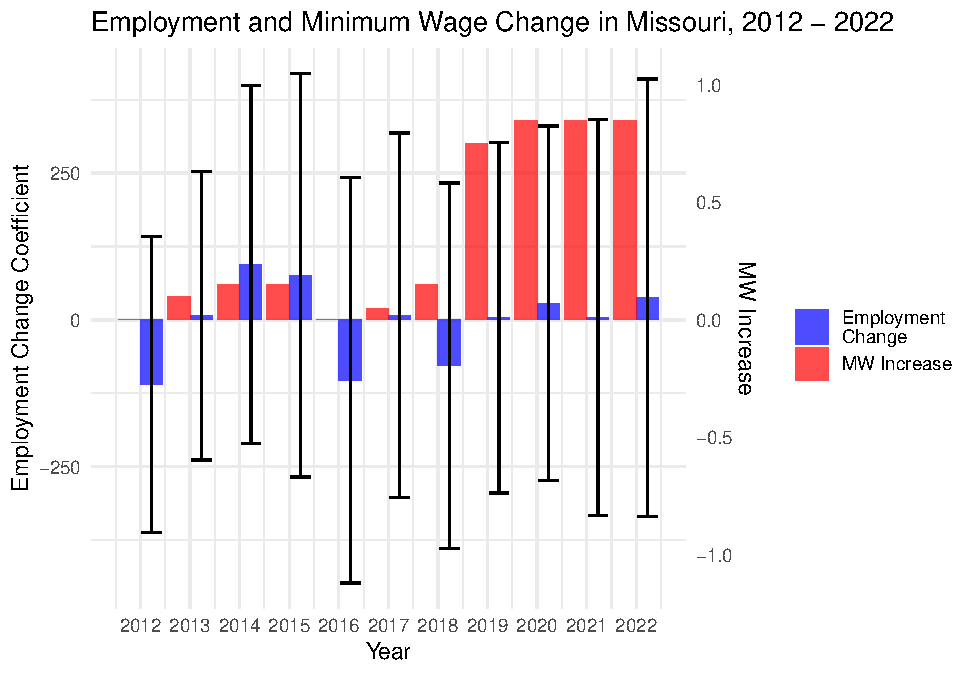
\includegraphics{regressions_files/figure-latex/unnamed-chunk-19-1.pdf}

\begin{Shaded}
\begin{Highlighting}[]
\CommentTok{\# Reshape the data into a longer format}
\NormalTok{reshaped\_data }\OtherTok{\textless{}{-}}\NormalTok{ Master\_Table }\SpecialCharTok{\%\textgreater{}\%}
  \FunctionTok{mutate}\NormalTok{(}\AttributeTok{mw\_increase =}\NormalTok{ mw\_increase}\SpecialCharTok{*}\NormalTok{(}\DecValTok{1}\SpecialCharTok{/}\FloatTok{0.0025}\NormalTok{)) }\SpecialCharTok{\%\textgreater{}\%}
  \FunctionTok{pivot\_longer}\NormalTok{(}
    \AttributeTok{cols =} \FunctionTok{c}\NormalTok{(state\_year\_coefficient, mw\_increase),}
    \AttributeTok{names\_to =} \StringTok{"Variable"}\NormalTok{,}
    \AttributeTok{values\_to =} \StringTok{"Value"}
\NormalTok{  )}

\CommentTok{\# Plotting the reshaped data}
\NormalTok{col\_plot }\OtherTok{\textless{}{-}} \FunctionTok{ggplot}\NormalTok{(reshaped\_data, }\FunctionTok{aes}\NormalTok{(}\AttributeTok{x =}\NormalTok{ year, }\AttributeTok{y =}\NormalTok{ Value, }\AttributeTok{fill =}\NormalTok{ Variable)) }\SpecialCharTok{+}
  \FunctionTok{geom\_col}\NormalTok{(}\AttributeTok{position =} \StringTok{"dodge"}\NormalTok{, }\AttributeTok{alpha =} \FloatTok{0.7}\NormalTok{) }\SpecialCharTok{+}
  \FunctionTok{geom\_errorbar}\NormalTok{(}\FunctionTok{aes}\NormalTok{(}\AttributeTok{ymin=}\NormalTok{ lwr, }\AttributeTok{ymax=}\NormalTok{ upr), }
                \AttributeTok{position =} \FunctionTok{position\_nudge}\NormalTok{( }\AttributeTok{x =} \FloatTok{0.23}\NormalTok{), }\AttributeTok{width =} \FloatTok{0.4}\NormalTok{) }\SpecialCharTok{+}
  \FunctionTok{labs}\NormalTok{(}
    \AttributeTok{title =} \StringTok{"Employment and Minimum Wage Change in Missouri, 2012 {-} 2022"}\NormalTok{,}
    \AttributeTok{x =} \StringTok{"Year"}\NormalTok{,}
    \AttributeTok{y =} \StringTok{"Values"}\NormalTok{,}
    \AttributeTok{fill =} \StringTok{" "}
\NormalTok{  ) }\SpecialCharTok{+} 
  \FunctionTok{scale\_fill\_manual}\NormalTok{(}\AttributeTok{values =} \FunctionTok{c}\NormalTok{(}\StringTok{"state\_year\_coefficient"} \OtherTok{=} \StringTok{"blue"}\NormalTok{, }\StringTok{"mw\_increase"} \OtherTok{=} \StringTok{"red"}\NormalTok{), }
                    \AttributeTok{breaks =} \FunctionTok{c}\NormalTok{(}\StringTok{"state\_year\_coefficient"}\NormalTok{, }\StringTok{"mw\_increase"}\NormalTok{),}
                    \AttributeTok{labels =} \FunctionTok{c}\NormalTok{(}\StringTok{"Employment}\SpecialCharTok{\textbackslash{}n}\StringTok{Change"}\NormalTok{, }\StringTok{"MW Increase"}\NormalTok{)) }\SpecialCharTok{+}
  \FunctionTok{scale\_y\_continuous}\NormalTok{(}
    \AttributeTok{name =} \StringTok{"Employment Change Coefficient"}\NormalTok{,}
    \AttributeTok{sec.axis =} \FunctionTok{sec\_axis}\NormalTok{(}\SpecialCharTok{\textasciitilde{}}\NormalTok{. }\SpecialCharTok{*}\NormalTok{ .}\DecValTok{0025}\NormalTok{, }\AttributeTok{name =} \StringTok{"MW Increase"}\NormalTok{)}
\NormalTok{  ) }\SpecialCharTok{+} 
  \FunctionTok{theme\_minimal}\NormalTok{() }\SpecialCharTok{+} 
  \FunctionTok{scale\_x\_continuous}\NormalTok{(}\AttributeTok{breaks =} \DecValTok{2012}\SpecialCharTok{:}\DecValTok{2022}\NormalTok{)}
  
\NormalTok{col\_plot}
\end{Highlighting}
\end{Shaded}

\includegraphics{regressions_files/figure-latex/unnamed-chunk-20-1.pdf}

\begin{Shaded}
\begin{Highlighting}[]
\FunctionTok{ggsave}\NormalTok{(}\AttributeTok{filename =} \StringTok{"Column\_Plot.png"}\NormalTok{, }\AttributeTok{plot =}\NormalTok{ col\_plot, }\AttributeTok{dpi =} \StringTok{"retina"}\NormalTok{, }\AttributeTok{width =} \FloatTok{10.4}\NormalTok{, }\AttributeTok{height =} \FloatTok{4.81}\NormalTok{)}
\end{Highlighting}
\end{Shaded}

\begin{Shaded}
\begin{Highlighting}[]
\FunctionTok{library}\NormalTok{(ggplot2)}
\FunctionTok{library}\NormalTok{(dplyr)}

\CommentTok{\# Set your desired scaling factor}
\NormalTok{scaling\_factor }\OtherTok{\textless{}{-}} \FloatTok{0.1}

\CommentTok{\# Create a long format of the data for ggplot}
\NormalTok{plot\_data }\OtherTok{\textless{}{-}}\NormalTok{ Coefficients\_visualizations\_table }\SpecialCharTok{\%\textgreater{}\%}
  \FunctionTok{pivot\_longer}\NormalTok{(}\AttributeTok{cols =} \FunctionTok{c}\NormalTok{(state\_year\_coefficient, mw\_increase),}
               \AttributeTok{names\_to =} \StringTok{"variable"}\NormalTok{,}
               \AttributeTok{values\_to =} \StringTok{"value"}\NormalTok{)}

\CommentTok{\# Create a grouped bar plot}
\FunctionTok{ggplot}\NormalTok{(plot\_data, }\FunctionTok{aes}\NormalTok{(}\AttributeTok{x =} \FunctionTok{as.factor}\NormalTok{(year), }\AttributeTok{fill =}\NormalTok{ variable, }\AttributeTok{y =}\NormalTok{ value)) }\SpecialCharTok{+}
  \FunctionTok{geom\_col}\NormalTok{(}\AttributeTok{position =} \StringTok{"dodge"}\NormalTok{, }\AttributeTok{alpha =} \FloatTok{0.7}\NormalTok{) }\SpecialCharTok{+}
  \FunctionTok{labs}\NormalTok{(}
    \AttributeTok{title =} \StringTok{"Grouped Bar Plot"}\NormalTok{,}
    \AttributeTok{x =} \StringTok{"Year"}\NormalTok{,}
    \AttributeTok{y =} \StringTok{"Values"}\NormalTok{,}
    \AttributeTok{fill =} \StringTok{"Legend"}
\NormalTok{  ) }\SpecialCharTok{+}
  \FunctionTok{scale\_fill\_manual}\NormalTok{(}\AttributeTok{values =} \FunctionTok{c}\NormalTok{(}\StringTok{"state\_year\_coefficient"} \OtherTok{=} \StringTok{"blue"}\NormalTok{, }\StringTok{"mw\_increase"} \OtherTok{=} \StringTok{"red"}\NormalTok{)) }\SpecialCharTok{+}
  \FunctionTok{facet\_wrap}\NormalTok{(}\SpecialCharTok{\textasciitilde{}}\NormalTok{ variable, }\AttributeTok{scales =} \StringTok{"free\_y"}\NormalTok{) }\SpecialCharTok{+}
  \FunctionTok{theme\_minimal}\NormalTok{()}
\end{Highlighting}
\end{Shaded}

\includegraphics{regressions_files/figure-latex/unnamed-chunk-21-1.pdf}

\begin{Shaded}
\begin{Highlighting}[]
\CommentTok{\#Regression Summaries for Table}

\FunctionTok{summary}\NormalTok{(model\_2011\_2012)}
\end{Highlighting}
\end{Shaded}

\begin{verbatim}
## 
## Call:
## lm(formula = emplvl_limited ~ state * year + emplvl_all, data = data_2011_2012)
## 
## Residuals:
##      Min       1Q   Median       3Q      Max 
## -1378.20  -259.06    11.75   253.85  1041.96 
## 
## Coefficients:
##                    Estimate Std. Error t value Pr(>|t|)    
## (Intercept)      -2.366e+02  7.564e+01  -3.128  0.00204 ** 
## stateMO           6.292e+02  9.366e+01   6.718 2.09e-10 ***
## year2012          1.272e+02  9.886e+01   1.287  0.19966    
## emplvl_all        3.070e-02  3.469e-04  88.510  < 2e-16 ***
## stateMO:year2012 -1.103e+02  1.276e+02  -0.864  0.38871    
## ---
## Signif. codes:  0 '***' 0.001 '**' 0.01 '*' 0.05 '.' 0.1 ' ' 1
## 
## Residual standard error: 435.3 on 190 degrees of freedom
## Multiple R-squared:  0.9765, Adjusted R-squared:  0.976 
## F-statistic:  1971 on 4 and 190 DF,  p-value: < 2.2e-16
\end{verbatim}

\begin{Shaded}
\begin{Highlighting}[]
\FunctionTok{summary}\NormalTok{(model\_2012\_2013)}
\end{Highlighting}
\end{Shaded}

\begin{verbatim}
## 
## Call:
## lm(formula = emplvl_limited ~ state * year + emplvl_all, data = data_2012_2013)
## 
## Residuals:
##      Min       1Q   Median       3Q      Max 
## -1123.55  -243.38   -25.84   244.83  1208.64 
## 
## Coefficients:
##                    Estimate Std. Error t value Pr(>|t|)    
## (Intercept)      -1.636e+02  7.374e+01  -2.218   0.0277 *  
## stateMO           5.490e+02  9.130e+01   6.013 9.14e-09 ***
## year2013          2.400e+01  9.636e+01   0.249   0.8036    
## emplvl_all        3.142e-02  3.305e-04  95.069  < 2e-16 ***
## stateMO:year2013  6.807e+00  1.244e+02   0.055   0.9564    
## ---
## Signif. codes:  0 '***' 0.001 '**' 0.01 '*' 0.05 '.' 0.1 ' ' 1
## 
## Residual standard error: 424.3 on 190 degrees of freedom
## Multiple R-squared:  0.9795, Adjusted R-squared:  0.9791 
## F-statistic:  2270 on 4 and 190 DF,  p-value: < 2.2e-16
\end{verbatim}

\begin{Shaded}
\begin{Highlighting}[]
\FunctionTok{summary}\NormalTok{(model\_2013\_2014)}
\end{Highlighting}
\end{Shaded}

\begin{verbatim}
## 
## Call:
## lm(formula = emplvl_limited ~ state * year + emplvl_all, data = data_2013_2014)
## 
## Residuals:
##     Min      1Q  Median      3Q     Max 
## -1332.2  -286.7  -139.9   309.9  1573.3 
## 
## Coefficients:
##                    Estimate Std. Error t value Pr(>|t|)    
## (Intercept)      -1.922e+02  9.175e+01  -2.095   0.0375 *  
## stateMO           5.966e+02  1.135e+02   5.254 3.96e-07 ***
## year2014         -3.232e+01  1.198e+02  -0.270   0.7877    
## emplvl_all        3.182e-02  4.030e-04  78.967  < 2e-16 ***
## stateMO:year2014  9.441e+01  1.547e+02   0.610   0.5424    
## ---
## Signif. codes:  0 '***' 0.001 '**' 0.01 '*' 0.05 '.' 0.1 ' ' 1
## 
## Residual standard error: 527.6 on 190 degrees of freedom
## Multiple R-squared:  0.9706, Adjusted R-squared:   0.97 
## F-statistic:  1568 on 4 and 190 DF,  p-value: < 2.2e-16
\end{verbatim}

\begin{Shaded}
\begin{Highlighting}[]
\FunctionTok{summary}\NormalTok{(model\_2014\_2015)}
\end{Highlighting}
\end{Shaded}

\begin{verbatim}
## 
## Call:
## lm(formula = emplvl_limited ~ state * year + emplvl_all, data = data_2014_2015)
## 
## Residuals:
##     Min      1Q  Median      3Q     Max 
## -1510.9  -314.4   -95.9   331.1  1636.3 
## 
## Coefficients:
##                    Estimate Std. Error t value Pr(>|t|)    
## (Intercept)      -2.536e+02  1.033e+02  -2.456    0.015 *  
## stateMO           6.958e+02  1.277e+02   5.448 1.56e-07 ***
## year2015          1.111e+01  1.348e+02   0.082    0.934    
## emplvl_all        3.191e-02  4.424e-04  72.128  < 2e-16 ***
## stateMO:year2015  7.599e+01  1.740e+02   0.437    0.663    
## ---
## Signif. codes:  0 '***' 0.001 '**' 0.01 '*' 0.05 '.' 0.1 ' ' 1
## 
## Residual standard error: 593.4 on 190 degrees of freedom
## Multiple R-squared:  0.965,  Adjusted R-squared:  0.9643 
## F-statistic:  1310 on 4 and 190 DF,  p-value: < 2.2e-16
\end{verbatim}

\begin{Shaded}
\begin{Highlighting}[]
\FunctionTok{summary}\NormalTok{(model\_2015\_2016)}
\end{Highlighting}
\end{Shaded}

\begin{verbatim}
## 
## Call:
## lm(formula = emplvl_limited ~ state * year + emplvl_all, data = data_2015_2016)
## 
## Residuals:
##      Min       1Q   Median       3Q      Max 
## -1745.90  -376.62    42.17   371.35  1632.88 
## 
## Coefficients:
##                    Estimate Std. Error t value Pr(>|t|)    
## (Intercept)      -3.129e+02  1.038e+02  -3.014  0.00293 ** 
## stateMO           8.244e+02  1.284e+02   6.420 1.06e-09 ***
## year2016          1.330e+02  1.355e+02   0.982  0.32757    
## emplvl_all        3.246e-02  4.366e-04  74.333  < 2e-16 ***
## stateMO:year2016 -1.029e+02  1.750e+02  -0.588  0.55719    
## ---
## Signif. codes:  0 '***' 0.001 '**' 0.01 '*' 0.05 '.' 0.1 ' ' 1
## 
## Residual standard error: 596.6 on 190 degrees of freedom
## Multiple R-squared:  0.967,  Adjusted R-squared:  0.9663 
## F-statistic:  1393 on 4 and 190 DF,  p-value: < 2.2e-16
\end{verbatim}

\begin{Shaded}
\begin{Highlighting}[]
\FunctionTok{summary}\NormalTok{(model\_2016\_2017)}
\end{Highlighting}
\end{Shaded}

\begin{verbatim}
## 
## Call:
## lm(formula = emplvl_limited ~ state * year + emplvl_all, data = data_2016_2017)
## 
## Residuals:
##      Min       1Q   Median       3Q      Max 
## -1382.61  -332.53    80.49   295.62  1443.59 
## 
## Coefficients:
##                    Estimate Std. Error t value Pr(>|t|)    
## (Intercept)      -2.373e+02  9.339e+01  -2.541   0.0119 *  
## stateMO           7.168e+02  1.155e+02   6.205 3.35e-09 ***
## year2017          6.643e+01  1.219e+02   0.545   0.5865    
## emplvl_all        3.276e-02  3.875e-04  84.541  < 2e-16 ***
## stateMO:year2017  7.615e+00  1.574e+02   0.048   0.9615    
## ---
## Signif. codes:  0 '***' 0.001 '**' 0.01 '*' 0.05 '.' 0.1 ' ' 1
## 
## Residual standard error: 536.8 on 190 degrees of freedom
## Multiple R-squared:  0.9743, Adjusted R-squared:  0.9737 
## F-statistic:  1799 on 4 and 190 DF,  p-value: < 2.2e-16
\end{verbatim}

\begin{Shaded}
\begin{Highlighting}[]
\FunctionTok{summary}\NormalTok{(model\_2017\_2018)}
\end{Highlighting}
\end{Shaded}

\begin{verbatim}
## 
## Call:
## lm(formula = emplvl_limited ~ state * year + emplvl_all, data = data_2017_2018)
## 
## Residuals:
##      Min       1Q   Median       3Q      Max 
## -1408.74  -368.25    67.68   265.23  1608.09 
## 
## Coefficients:
##                    Estimate Std. Error t value Pr(>|t|)    
## (Intercept)      -1.686e+02  9.361e+01  -1.801   0.0733 .  
## stateMO           7.311e+02  1.158e+02   6.314 1.88e-09 ***
## year2018          2.347e+01  1.222e+02   0.192   0.8479    
## emplvl_all        3.204e-02  3.825e-04  83.770  < 2e-16 ***
## stateMO:year2018 -7.805e+01  1.578e+02  -0.495   0.6214    
## ---
## Signif. codes:  0 '***' 0.001 '**' 0.01 '*' 0.05 '.' 0.1 ' ' 1
## 
## Residual standard error: 538.1 on 190 degrees of freedom
## Multiple R-squared:  0.9738, Adjusted R-squared:  0.9732 
## F-statistic:  1765 on 4 and 190 DF,  p-value: < 2.2e-16
\end{verbatim}

\begin{Shaded}
\begin{Highlighting}[]
\FunctionTok{summary}\NormalTok{(model\_2018\_2019)}
\end{Highlighting}
\end{Shaded}

\begin{verbatim}
## 
## Call:
## lm(formula = emplvl_limited ~ state * year + emplvl_all, data = data_2018_2019)
## 
## Residuals:
##     Min      1Q  Median      3Q     Max 
## -1302.1  -425.4   125.8   373.5  1256.1 
## 
## Coefficients:
##                    Estimate Std. Error t value Pr(>|t|)    
## (Intercept)      -1.462e+02  8.971e+01  -1.630    0.105    
## stateMO           6.716e+02  1.110e+02   6.051 7.52e-09 ***
## year2019          4.411e+01  1.171e+02   0.377    0.707    
## emplvl_all        3.130e-02  3.625e-04  86.354  < 2e-16 ***
## stateMO:year2019  3.542e+00  1.512e+02   0.023    0.981    
## ---
## Signif. codes:  0 '***' 0.001 '**' 0.01 '*' 0.05 '.' 0.1 ' ' 1
## 
## Residual standard error: 515.8 on 190 degrees of freedom
## Multiple R-squared:  0.9753, Adjusted R-squared:  0.9748 
## F-statistic:  1876 on 4 and 190 DF,  p-value: < 2.2e-16
\end{verbatim}

\begin{Shaded}
\begin{Highlighting}[]
\FunctionTok{summary}\NormalTok{(model\_2019\_2020)}
\end{Highlighting}
\end{Shaded}

\begin{verbatim}
## 
## Call:
## lm(formula = emplvl_limited ~ state * year + emplvl_all, data = data_2019_2020)
## 
## Residuals:
##     Min      1Q  Median      3Q     Max 
## -1704.0  -431.7   108.5   358.8  1431.2 
## 
## Coefficients:
##                    Estimate Std. Error t value Pr(>|t|)    
## (Intercept)      -1.323e+02  9.090e+01  -1.455    0.147    
## stateMO           6.983e+02  1.122e+02   6.224 3.03e-09 ***
## year2020         -6.167e+00  1.184e+02  -0.052    0.959    
## emplvl_all        3.176e-02  3.743e-04  84.843  < 2e-16 ***
## stateMO:year2020  2.862e+01  1.529e+02   0.187    0.852    
## ---
## Signif. codes:  0 '***' 0.001 '**' 0.01 '*' 0.05 '.' 0.1 ' ' 1
## 
## Residual standard error: 521.3 on 190 degrees of freedom
## Multiple R-squared:  0.9745, Adjusted R-squared:  0.9739 
## F-statistic:  1812 on 4 and 190 DF,  p-value: < 2.2e-16
\end{verbatim}

\begin{Shaded}
\begin{Highlighting}[]
\FunctionTok{summary}\NormalTok{(model\_2020\_2021)}
\end{Highlighting}
\end{Shaded}

\begin{verbatim}
## 
## Call:
## lm(formula = emplvl_limited ~ state * year + emplvl_all, data = data_2020_2021)
## 
## Residuals:
##      Min       1Q   Median       3Q      Max 
## -1476.92  -505.88    71.44   426.61  1399.53 
## 
## Coefficients:
##                    Estimate Std. Error t value Pr(>|t|)    
## (Intercept)      -1.484e+02  1.014e+02  -1.464    0.145    
## stateMO           8.073e+02  1.254e+02   6.438 9.66e-10 ***
## year2021         -2.957e+01  1.323e+02  -0.223    0.823    
## emplvl_all        3.162e-02  4.264e-04  74.156  < 2e-16 ***
## stateMO:year2021  4.472e+00  1.709e+02   0.026    0.979    
## ---
## Signif. codes:  0 '***' 0.001 '**' 0.01 '*' 0.05 '.' 0.1 ' ' 1
## 
## Residual standard error: 582.7 on 190 degrees of freedom
## Multiple R-squared:  0.9669, Adjusted R-squared:  0.9662 
## F-statistic:  1388 on 4 and 190 DF,  p-value: < 2.2e-16
\end{verbatim}

\begin{Shaded}
\begin{Highlighting}[]
\FunctionTok{summary}\NormalTok{(model\_2021\_2022)}
\end{Highlighting}
\end{Shaded}

\begin{verbatim}
## 
## Call:
## lm(formula = emplvl_limited ~ state * year + emplvl_all, data = data_2021_2022)
## 
## Residuals:
##     Min      1Q  Median      3Q     Max 
## -1752.3  -519.3   151.8   396.1  1595.8 
## 
## Coefficients:
##                    Estimate Std. Error t value Pr(>|t|)    
## (Intercept)      -2.067e+02  1.119e+02  -1.847   0.0664 .  
## stateMO           8.502e+02  1.385e+02   6.137  4.8e-09 ***
## year2022          2.490e+01  1.462e+02   0.170   0.8650    
## emplvl_all        3.113e-02  4.556e-04  68.330  < 2e-16 ***
## stateMO:year2022  3.783e+01  1.888e+02   0.200   0.8414    
## ---
## Signif. codes:  0 '***' 0.001 '**' 0.01 '*' 0.05 '.' 0.1 ' ' 1
## 
## Residual standard error: 643.7 on 190 degrees of freedom
## Multiple R-squared:  0.9613, Adjusted R-squared:  0.9605 
## F-statistic:  1180 on 4 and 190 DF,  p-value: < 2.2e-16
\end{verbatim}

\begin{Shaded}
\begin{Highlighting}[]
\FunctionTok{library}\NormalTok{(stargazer)}
\end{Highlighting}
\end{Shaded}

\begin{verbatim}
## 
## Please cite as:
\end{verbatim}

\begin{verbatim}
##  Hlavac, Marek (2022). stargazer: Well-Formatted Regression and Summary Statistics Tables.
\end{verbatim}

\begin{verbatim}
##  R package version 5.2.3. https://CRAN.R-project.org/package=stargazer
\end{verbatim}

\begin{Shaded}
\begin{Highlighting}[]
\NormalTok{table\_models }\OtherTok{\textless{}{-}} \FunctionTok{list}\NormalTok{(model\_2011\_2012, model\_2012\_2013, model\_2013\_2014, model\_2014\_2015, model\_2015\_2016, model\_2016\_2017, model\_2017\_2018, model\_2018\_2019, model\_2019\_2020, model\_2020\_2021, model\_2021\_2022)}
\end{Highlighting}
\end{Shaded}

\begin{Shaded}
\begin{Highlighting}[]
\NormalTok{model\_names }\OtherTok{\textless{}{-}} \FunctionTok{c}\NormalTok{(}\StringTok{"Model 2011{-}2012"}\NormalTok{, }\StringTok{"Model 2012{-}2013"}\NormalTok{, }\StringTok{"Model 2013{-}2014"}\NormalTok{, }\StringTok{"Model 2014{-}2015"}\NormalTok{, }\StringTok{"Model 2015{-}2016"}\NormalTok{, }\StringTok{"Model 2016{-}2017"}\NormalTok{, }\StringTok{"Model 2017{-}2018"}\NormalTok{, }\StringTok{"Model 2018{-}2019"}\NormalTok{, }\StringTok{"Model 2019{-}2020"}\NormalTok{, }\StringTok{"Model 2020{-}2021"}\NormalTok{, }\StringTok{"Model 2021{-}2022"}\NormalTok{)}

\CommentTok{\# Extract coefficients for each model}
\NormalTok{coefficients\_list }\OtherTok{\textless{}{-}} \FunctionTok{lapply}\NormalTok{(table\_models, coef)}

\CommentTok{\# Create a new list to store consolidated coefficients}
\NormalTok{consolidated\_coefficients }\OtherTok{\textless{}{-}} \FunctionTok{list}\NormalTok{()}

\CommentTok{\# Loop through each year}
\ControlFlowTok{for}\NormalTok{ (year }\ControlFlowTok{in} \FunctionTok{unique}\NormalTok{(}\FunctionTok{gsub}\NormalTok{(}\StringTok{".*year(.*)"}\NormalTok{, }\StringTok{"}\SpecialCharTok{\textbackslash{}\textbackslash{}}\StringTok{1"}\NormalTok{, }\FunctionTok{names}\NormalTok{(coefficients\_list[[}\DecValTok{1}\NormalTok{]])))) \{}
  \CommentTok{\# Extract coefficients for the specific year}
\NormalTok{  year\_coefficients }\OtherTok{\textless{}{-}} \FunctionTok{lapply}\NormalTok{(coefficients\_list, }\ControlFlowTok{function}\NormalTok{(model) model[}\FunctionTok{grep}\NormalTok{(}\FunctionTok{paste0}\NormalTok{(}\StringTok{"year"}\NormalTok{, year), }\FunctionTok{names}\NormalTok{(model))])}
  
  \CommentTok{\# Consolidate coefficients for the specific year}
\NormalTok{  consolidated\_coefficients[[year]] }\OtherTok{\textless{}{-}} \FunctionTok{do.call}\NormalTok{(cbind, year\_coefficients)}
\NormalTok{\}}
\end{Highlighting}
\end{Shaded}

\begin{Shaded}
\begin{Highlighting}[]
\CommentTok{\# Customize stargazer options}
\FunctionTok{stargazer}\NormalTok{(}
\NormalTok{  table\_models[[}\DecValTok{1}\NormalTok{]],}
  \AttributeTok{title =} \StringTok{"Regression Results"}\NormalTok{,}
  \AttributeTok{type =} \StringTok{\textquotesingle{}latex\textquotesingle{}}\NormalTok{,}
  \AttributeTok{align =} \ConstantTok{TRUE}\NormalTok{,                  }\CommentTok{\# Align coefficient names to the left}
  \AttributeTok{dep.var.caption =} \StringTok{"Dependent variable: }\SpecialCharTok{\textbackslash{}\textbackslash{}}\StringTok{textbf\{emplvl}\SpecialCharTok{\textbackslash{}\textbackslash{}}\StringTok{\_limited\}"}\NormalTok{,  }\CommentTok{\# Bold dependent variable in the caption}
  \AttributeTok{column.labels =}\NormalTok{ model\_names,   }\CommentTok{\# Model labels}
  \AttributeTok{covariate.labels =} \FunctionTok{names}\NormalTok{(consolidated\_coefficients[[}\DecValTok{1}\NormalTok{]]),  }\CommentTok{\# Custom order of variables}
  \AttributeTok{digits =} \DecValTok{3}\NormalTok{,                    }\CommentTok{\# Number of decimal places}
  \AttributeTok{star.cutoffs =} \FunctionTok{c}\NormalTok{(}\FloatTok{0.1}\NormalTok{, }\FloatTok{0.05}\NormalTok{, }\FloatTok{0.01}\NormalTok{),  }\CommentTok{\# Customize significance stars}
  \AttributeTok{notes =} \StringTok{"}\SpecialCharTok{\textbackslash{}\textbackslash{}}\StringTok{textit\{Note:\} $\^{}\{*\}p\textless{}0.1; \^{}\{**\}p\textless{}0.05; \^{}\{***\}p\textless{}0.01"}\NormalTok{,  }\CommentTok{\# Custom note}
  \AttributeTok{omit =} \FunctionTok{names}\NormalTok{(consolidated\_coefficients[[}\DecValTok{1}\NormalTok{]])[}\SpecialCharTok{{-}}\DecValTok{1}\NormalTok{]  }\CommentTok{\# Omit redundant coefficients}
\NormalTok{)}
\end{Highlighting}
\end{Shaded}

\% Table created by stargazer v.5.2.3 by Marek Hlavac, Social Policy
Institute. E-mail: marek.hlavac at gmail.com \% Date and time: Mon, Dec
11, 2023 - 9:48:12 PM \% Requires LaTeX packages: dcolumn

\begin{table}[!htbp] \centering 
  \caption{Regression Results} 
  \label{} 
\begin{tabular}{@{\extracolsep{5pt}}lD{.}{.}{-3} } 
\\[-1.8ex]\hline 
\hline \\[-1.8ex] 
 & \multicolumn{1}{c}{Dependent variable: \textbf{emplvl\_limited}} \\ 
\cline{2-2} 
\\[-1.8ex] & \multicolumn{1}{c}{emplvl\_limited} \\ 
 & \multicolumn{1}{c}{Model 2011-2012} \\ 
\hline \\[-1.8ex] 
 stateMO & 629.192^{***} \\ 
  & (93.663) \\ 
  & \\ 
 year2012 & 127.233 \\ 
  & (98.859) \\ 
  & \\ 
 emplvl\_all & 0.031^{***} \\ 
  & (0.0003) \\ 
  & \\ 
 stateMO:year2012 & -110.262 \\ 
  & (127.627) \\ 
  & \\ 
 Constant & -236.602^{***} \\ 
  & (75.642) \\ 
  & \\ 
\hline \\[-1.8ex] 
Observations & \multicolumn{1}{c}{195} \\ 
R$^{2}$ & \multicolumn{1}{c}{0.976} \\ 
Adjusted R$^{2}$ & \multicolumn{1}{c}{0.976} \\ 
Residual Std. Error & \multicolumn{1}{c}{435.258 (df = 190)} \\ 
F Statistic & \multicolumn{1}{c}{1,971.273$^{***}$ (df = 4; 190)} \\ 
\hline 
\hline \\[-1.8ex] 
\textit{Note:}  & \multicolumn{1}{r}{$^{*}$p$<$0.1; $^{**}$p$<$0.05; $^{***}$p$<$0.01} \\ 
 & \multicolumn{1}{r}{\textit{Note:} $^{*}p<0.1; ^{**}p<0.05; ^{***}p<0.01} \\ 
\end{tabular} 
\end{table}

\begin{Shaded}
\begin{Highlighting}[]
\CommentTok{\# Trying with the three year pairs instead}

\NormalTok{table\_models\_2 }\OtherTok{\textless{}{-}} \FunctionTok{list}\NormalTok{(model\_2011\_2012, model\_2012\_2013, model\_2013\_2014)}


\CommentTok{\# stargazer(table\_models\_2)}
\end{Highlighting}
\end{Shaded}


\end{document}
